\documentclass[a0paper,portrait]{baposter}
\usepackage[utf8]{inputenc}

\usepackage{relsize}                  % For \smaller
\usepackage{url}  % For \url
\usepackage{tikz}  % To draw background
\usepackage{booktabs}

%%% Global Settings %%%%%%%%%%%%%%%%%%%%%%%%%%%%%%%%%%%%%%%%%%%%%%%%%%%%%%%%%%%

\graphicspath{{figures/}}            % Root directory of the pictures 

%%% Color Definitions %%%%%%%%%%%%%%%%%%%%%%%%%%%%%%%%%%%%%%%%%%%%%%%%%%%%%%%%%

% Those are the official imperial colours:
\definecolor{Navy}{RGB}{0,33,71}
\definecolor{ImperialBlue}{RGB}{0,62,116}
\definecolor{LightGrey}{RGB}{235,238,238}
\definecolor{CoolGrey}{RGB}{157,157,157}
\definecolor{LightBlue}{RGB}{212,239,252}
\definecolor{Black}{RGB}{0,0,0}
\definecolor{White}{RGB}{255,255,255}

%%%%%%%%%%%%%%%%%%%%%%%%%%%%%%%%%%%%%%%%%%%%%%%%%%%%%%%%%%%%%%%%%%%%%%%%%%%%%%%% 
%%% Utility functions %%%%%%%%%%%%%%%%%%%%%%%%%%%%%%%%%%%%%%%%%%%%%%%%%%%%%%%%%%

%%% Save space in lists. Use this after the opening of the list %%%%%%%%%%%%%%%%
\newcommand{\compresslist}{
  \setlength{\itemsep}{3pt}
  \setlength{\parskip}{2pt}
  \setlength{\parsep}{2pt}

\vspace{-0.75em}

}

\newcommand{\tab}{\hspace{0.5em}}

%%%%%% Author Affiliations %%%
\newcommand{\footremember}[2]{%
    \footnote{#2}
    \newcounter{#1}
    \setcounter{#1}{\value{footnote}}%
}
\newcommand{\footrecall}[1]{%
    \footnotemark[\value{#1}]%
} 

\usepackage[backend=biber, sorting=nty, style=ieee, minbibnames=1, maxbibnames=1, maxcitenames=1, mincitenames=1, defernumbers=true]{biblatex}
\addbibresource{nips_2016.bib}
%\addbibresource{websites.bib}

\AtEveryBibitem{%
  \clearfield{url}%
  \clearfield{doi}%
  \clearfield{issn}
  \clearfield{volume}
  \clearfield{number}
  \clearfield{pages}
  \clearfield{isbn}
  \clearfield{eprint}
}

\DefineBibliographyStrings{english}{%
  references = {},
}

\renewcommand\refname{}


\begin{document}
%%% Setting Background Image %%%%%%%%%%%%%%%%%%%%%%%%%%%%%%%%%%%%%%%%%%%%%%%%%%

\background{
  % Change colours of body background and header background if desired
  % you can also use tikz to include a custom picture here
  \begin{tikzpicture}[remember picture,overlay]%
    %the poster background colour
    \fill[fill=LightGrey] (current page.north west) rectangle (current page.south east);
    %the header
    \fill [fill=LightGrey] (current page.north west) rectangle ([yshift=-\headerheight] current page.north east);
  \end{tikzpicture}
}

\begin{poster}{
  grid=false,
  eyecatcher=true, 
  borderColor=White,
  headerColorOne=ImperialBlue,
  headerColorTwo=ImperialBlue,
  headerFontColor=LightGrey,
  boxColorOne=White,
  headershape=roundedright,
  textborder=roundedleft,
  background=user,
  headerborder=none, 
  textborder=none,
  boxshade=plain,
  headerheight=100pt
}
%%% Eye Cacther %%%%%%%%%%%%%%%%%%%%%%%%%%%%%%%%%%%%%%%%%%%%%%%%%%%%%%%%%%%%%%%
{
  %\vspace{-20pt}
  %\includegraphics[width=0.15\textwidth]{broad}
}
%%% Title %%%%%%%%%%%%%%%%%%%%%%%%%%%%%%%%%%%%%%%%%%%%%%%%%%%%%%%%%%%%%%%%%%%%%
{
  {\sf\bf \textcolor{Black}{Automating Morphological Profiling with Generic Deep Convolutional Networks}}
  \vspace{3pt} % move authors list down a little bit
} 
%%% Authors %%%%%%%%%%%%%%%%%%%%%%%%%%%%%%%%%%%%%%%%%%%%%%%%%%%%%%%%%%%%%%%%%%%
{
  \textcolor{Black}{Nick Pawlowski$^{1}$, Juan C Caicedo$^{2}$, Shantanu Singh$^{2}$, Anne E Carpenter$^{2}$, Amos Storkey$^{3}$}\\
  \vspace{3pt} \smaller[2] \textcolor{Black}{(1) Imperial College (previously (3)), (2) Broad Institute, (3) University of Edinburgh}
  %\textcolor{Black}{np716@imperial.ac.uk, \{jccaicedo, shsingh, anne\}@broadinstitute.org, a.storkey@ed.ac.uk}
}
%%% Logo %%%%%%%%%%%%%%%%%%%%%%%%%%%%%%%%%%%%%%%%%%%%%%%%%%%%%%%%%%%%%%%%%%%%%%
{
  %\vspace{-20pt}
  \includegraphics[width=0.2\textwidth]{logos}
}

\headerbox{1: Motivation}{name=motivation,column=0,row=0}{

Morphological profiling aims to create {\bf profiles} or signatures of genes, chemicals and diseases from microscopy images. These signatures have several applications, including
\begin{itemize}
\compresslist
\item functional genomics
\item drug discovery
\item target identification
\end{itemize}
Current approaches need human supervision to fine-tune parameters of classical algorithms to extract meaningful features from images \cite{caicedo_profiling}. We propose the use of pre-trained deep convolutional networks for feature extraction. Our contributions are:
\begin{itemize}
\compresslist
\item \textbf{Speed}: It enables faster profile computation than the classical pipeline with image segmentation and feature extraction.
\item \textbf{Autonomous}: It eliminates the need for human input to tune parameters.
\item \textbf{Performance}: The extracted profiles achieve a better accuracy than a baseline approach based on handcrafted features.
\end{itemize}
}

\headerbox{2: Overview}{name=overview, span=2, column=1, row=0}{

Activations of pre-trained neural network constitute profiles for individual images. Profiles from images of the same treatment are averaged to form a treatment (i.e. gene, chemical, or disease) profile.


\begin{minipage}[c]{\textwidth}
	\centering
	\includegraphics[width=0.95\textwidth]{overview3}
\end{minipage}
\\
\\
By measuring similarities or distances between these profiles in this representation space, they can be used to find relationships between the treatments – a valuable tool when investigating the function of a gene or allele, figuring out the mechanism of action of a compound, relating the phenotype of a disease with that of a genetic or chemical treatment, and many questions. 
}

\headerbox{3: Representation Space}{name=rep, span=1, column=0, row=1, below=motivation}{

On an example dataset, the extracted profiles from neural networks span a representation space with mostly clear clusters regarding the biological mechanism-of-action. Inception-v3 extracted profiles can be visualised using t-SNE.
\\
\\
\begin{minipage}[c]{\textwidth}
	\centering
	\includegraphics[width=1.0\textwidth]{tsne}
\end{minipage}
\\
\\
Inception-v3 profiles show the best clustering of biological mechanisms-of-action of the tested compounds.
}

\headerbox{4: Mechanism-of-Action Classification}{name=results, span=2, column=1, row=1, below=overview}{

Classification results using different pre-trained neural networks with different types of images. The neural networks were pre-trained on the ImageNet dataset. The full-sized images were resized to the appropriate input size of the neural network. Greyscale images account for the use of each greyscale channel as separate image. Illum corrected images use the technique proposed by Singh et al.\cite{Singh2014} to compensate for illumination bias during microscopy imaging. We use 1NN classification leaving out profiles from the same compound.
\\
\\
\begin{minipage}[c]{\textwidth}
   \centering
\begin{tabular}{l|rrrr}
\toprule
 & Inception-v3\cite{Szegedy2015} & ResNet-152\cite{He2015} & ResNet-101\cite{He2015} & VGG 16\cite{Simonyan2015}\\
\midrule
Full Images & $70.87\%$ &  $55.34\%$ & $57.28\%$ & $66.02\%$\\
+ illum corrected & $69.90\%$ & $65.05\%$ & $65.04\%$ & $63.11\%$ \\
+ greyscale & $86.41\%$ & $75.72\%$ & $70.87\%$ & $71.84\%$ \\
+ illum corrected \& greyscale  & \textbf{$91.26\%$} & $78.64\%$ & $79.61\%$ & $83.50\%$\\
\bottomrule
\end{tabular}
\end{minipage}
\\
\\
Confusion matrices for the Inception-v3 extracted profiles (left) show an improvement over the classical results (right)\cite{Singh2014}:
\\
\\
\begin{minipage}[c]{\textwidth}
	\centering
	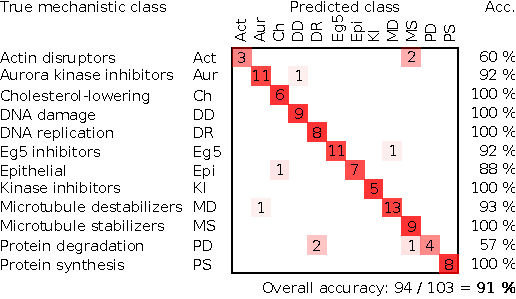
\includegraphics[width=0.45\textwidth]{eval_inception_full_images_illumcorr_channelasimg.pdf}
    \hfill
    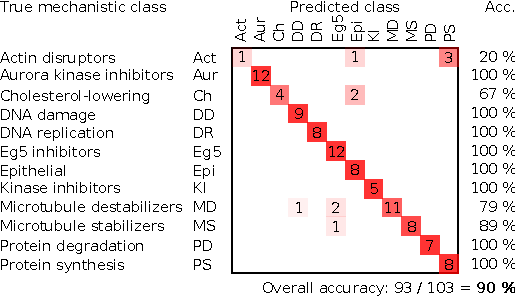
\includegraphics[width=0.45\textwidth]{mean_treatment_confusion.pdf}
\end{minipage}
\\
\\
The  different confusion matrices show that complimentary information is present in both profile types. 
}



\headerbox{5: Dose Response}{name=dose, span=2, column=1, row=2, below=results}{

The extracted profiles can be evaluated according to the dose response curves. Some compounds show chaotic relations (left). However, other compounds exhibit the expected direct relation between higher dose and stronger response (right).
\\
\begin{minipage}[c]{\textwidth}
	\centering
	\includegraphics[width=0.45\textwidth]{floxuridine_dose}
    \hfill
    \includegraphics[width=0.45\textwidth]{mitoxantrone_dose}
\end{minipage}

}

\headerbox{Acknowledgements}{name=ack, span=1, column=2, row=4, below=dose}{

We want to thank Mike Ando (Google, Inc.) for helpful discussions about the use of transfer learning for the domain of morphological profiling. We want to thank all members of the Imaging Platform for helpful discussions. AEC acknowledges NSF support (NSF CAREER DBI 1148823 to AEC).

}

\headerbox{Code \& Dataset}{name=Note, span=1, column=1, row=4, below=dose}{

Code is available at \url{github.com/carpenterlab/2016_pawlowski_mlcb}.\\
Dataset is available as BBBC021 of the Broad Bioimage Benchmark Collection at \url{data.broadinstitute.org/bbbc/BBBC021/}.\\
\vspace*{1.5em}
}

\headerbox{References}{name=References, span=1, column=0, row=4, below=rep}{
\vspace*{-1.5em}
\printbibliography
\vspace*{0.65em}
}

\end{poster}
\end{document}
